\documentclass{article}
\usepackage[margin=1in]{geometry}
\usepackage{graphicx}
\usepackage{a4wide}
\usepackage{float}
\usepackage{listings}

\graphicspath{graphics}

\begin{document}
\title{Report --- Juniour Honours Project Submission 1}
\author{Hafeez Abdul-Rehaman, Johannes Weck, Josh Lee, Calum Duff, Tom Harley}
\date{\today}

\maketitle

\tableofcontents

\section{Requirements Overview}
For our Junior Honours project, we are to design and create a database
for a system which will be used primarily for the sharing and viewing
of various medical and pathological media.

Our database is to be:
\begin{description}
  \item[User-aware] The system should act as a platform for managing
    users and their permissions, with respect to viewing and affecting
    projects and media.
  \item[Filetype-agnostic] The system should accept files in a
    variety of filetypes and be able to translate between them, in order to
    provide a user with a desirable output filetype.
  \item[Substitutable] The system should follow standardised
    communication protocols, to participate in a framework of modularised
    systems created in conjunction with other Junior Honours groups.
\end{description}

\section{Using Scrum}
The Scrum approach facilitated the
planning and running of group meetings. As the year-wide protocol changed
over time, an AGILE working process provided the granular iteration
required to address the frequent design changes.

\subsection{Scrum Board}
Throughout the project a Scrum board has been used to keep track of current tasks
and further items to implement. A whiteboard in the John Honey main computer lab
was used throughout this process. Examples of the board in use can be found in
Appendix \ref{app:board}.

The Scrum board made visualizing tasks and progression straightforward.
Using it in meetings helped with determining how much was still to be done.

At times the \emph{In Progress} section of the Scrum board seemed unbalanced;
at these times several people were working on the same large task, and so fewer
notes were placed in this column.

\subsection{Time Management}
Based on how tasks were split, and the difficulty of various tasks, we estimated
durations for each task. Due to the widely-varying estimated completion times,
we decided to distribute our Sprint durations accordingly.
Initially, we divided our total available time with the number of available tasks,
but over time experience from previous work and from previous meetings was helpful in
refining the expected duration of the future tasks.
This, combined with
the late reveal of the specification meant that work was done over holidays, greatly 
warping the duration of several Sprints to be longer than anticipated.

\begin{figure}[H]
\centering
    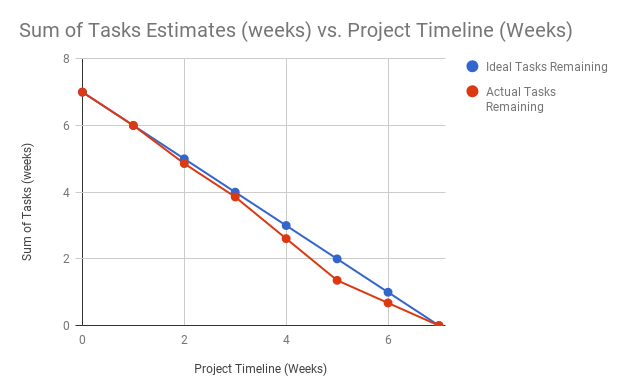
\includegraphics[width=\linewidth]{graphics/chart.png}
    \caption{A Burn Down chart graphically representing average completion time of tasks}
    \label{fig:burndown}
\end{figure}

\subsection{Meetings}
Meetings were held every 1-3 weeks with the entire team.
They were carried out in person or, during the holidays, using
voice chat clients.

Meetings helped members of the team understand what was being done by
other members of the team, particularly in areas were only one person
was working. They also helped the team decide on what was important to
attempt in the next Sprint.

The minutes for formal meetings are available in Appendix \ref{app:meet}.

\subsection{Paired Programming/Teamwork}
Paired Programming was used extensively throughout implementation of basic server
functions, such as writing logic for the public protocol endpoints.

Multiple people working on a single task reduces the total actual time it takes to
complete. This allowed larger tasks that would not normally fit into a regular Sprint
to still be tackled within a single Sprint.

At times the entire team was in labs, working concurrently on separate tasks.

Having everyone in the same place focussed everyone on the task at hand and greatly
improved communication, keeping everyone working on what was important and not dallying.

\subsection{Evaluation of Work Done/To Do}
The Scrum board and regular meetings greatly aided in our evaluation of how much work
had been completed, and how much there was left to do, at the time. Now that we're
used to Scrum, evaluation of further tasks (such as extensions) should be more
realistic, and tasks are more likely to be assigned to Sprints with enough time to
accommodate them, instead of persisting to the next Sprint.

\section{Design Decisions}
\subsection{Database}
\subsubsection{Security}
Passwords in the database are currently stored totally unencrypted. Initially,
the focus of work was on routing traffic, and for this purpose salting
passwords is unnecessary. Once the server is past development phase, passwords
will be encrypted in some secure fashion.

\subsubsection{File Representation}
File paths are stored in the database, represented as one-to-many parent-folder-to-file
mappings. This decision was made since all files will already have entries in the
database (such as metadata and their UUID), and adding the remainder of necessary
information for a file would be simple.

While file paths are stored in the database, the file content itself will not be.
It has been specified that the system should be capable of storing large files,
and databases may struggle with the difficulties of storing variable-size Binary
Large Objects when said objects are of this scale. In addition, the breakdown and
caching of large images into image pyramids both increases the quantity of binary
data that will need to be stored, and greatly increases the number of reads and
writes carried out by the server on binary data. File systems, on the other hand,
are optimised for jobs of this kind.

The resulting setup is a virtual filesystem that resembles a regular filesystem,
and a very flat physical filesystem: a root folder containing a folder for each
project, which in turn contain all non-folder files belonging to that particular project.
Keeping the files separated by folders named after their projects allows for simple
deletion of an entire project.

All files in the database are given a UUID, which serves a number of functions:
\begin{enumerate}
    \item It is the name of the file in the physical file system on disk,
    \item It can be used to uniquely identify a file irrespective of its position
        in the virtual file system,
    \item It can be used to keep a reference to a file even if it is moved
        (or even if it is deleted).
\end{enumerate}

Examples of SQL queries using the structure described can be found in Appendix
\ref{app:sql}.

\subsection{Server Framework}
This practical requires a variety of utilities, and should be easy to document and
to understand from an outside perspective. Additionally, it was decided that for a
large project a language and platform that all members of the team were comfortable
with was a high priority. Finally, the system would need to be scalable, in the sense
that additional features should be easy to implement and plug in to the
already-functioning system.

For these reasons, NodeJS and Typescript were chosen as the framework and language
for the project.

\subsubsection{NodeJS}
NodeJS has a huge library (or \emph{package}) repository, providing teams with a wide variety of options on how to implement projects. Its ease of deployment on both *nix and Windows systems,
and its common IDE support make it ideal for team development.

\subsubsection{Typescript}
While not every team member had previously used Typescript, all had used and are comfortable
with Javascript, and were willing to take on the slight increase in complexity for static
type checking. Typescript's compile-time checks and IDE integration remove the ambiguity of
Javascript from large projects, improving their scalability and maintainability as the project
increases in size.

\subsubsection{ExpressJS}
A core package used by the project for client-server communication is the middleware handler
ExpressJS. This package allows for easy insertion and use of any number of middlewares, both created in-house
and imported from other packages. Uses for this multi-layer structure include authentication, user
permission checking, and wrapping responses with statuses.

ExpressJS also handles client-server communication through a RESTful API.

\begin{figure}[H]
    \centering
    \includegraphics[width=1.5in]{graphics/be-layer-structure.pdf}
    \caption{Structure of Layers in a Server Instance}
    \label{fig:layer}
\end{figure}

\subsubsection{Sequelize (and Sequelize-Typescript)}
Sequelize was chosen as the ORM package to use to connect to the database server. It was chosen over other
similar packages for its variety of powerful features (such as eager loading) and its large user-base.
It can connect to a variety of SQL-dialect databases, and hides the low-level table interactions to create
a simple abstraction to Javascript objects.
Furthermore, it also has comprehensive and clear documentation, providing better access to these features.

In addition to Sequelize is the add-on package Sequelize-Typescript: this improves Sequelize syntax to
accept ES6 classes with Typescript types as ORM model definitions, amongst other smaller improvements
made possible by Typescript's experimental annotation support.

\subsubsection{Token-Based Authentication (Passport/JWT)}
The protocol designed by the entire year uses a token-based authentication service
similar to and inspired by OAuth2. Using token-based authentication removes the need
for sessions or for cookies while still providing a smooth and secure user experience,
and simplifying client design.
It was decided that implementing OAuth2 in its entirety would be superfluous. OAuth2
relies on the acquisition of tokens from third parties, which would be unsuitable for
a simple system such as this.

The Javascript package Passport was used for handling authentication through this protocol.
Passport's support for custom authentication services in addition to its synergy with ExpressJS middleware
support made it an obvious choice.

For generating authentication "bearer" tokens, JWT was used.

\subsection{Testing Framework}
Testing was extensive and concurrent to the implementation in each Sprint. This was to ensure minimal time was spent debugging which then prevented the team from missing the Sprint deadlines. Unit testing was one of the primary methods of testing individual functionality. This was very useful for a modularised task as each module could be debugged without affecting other modules which were functioning as expected. Producing unit tests concurrently with the implementation of certain functionality gave the advantage of designing the functionality around the possible input or validation errors that may occur. MochaJS and ChaiJS were the JavaScript frameworks used for unit testing. These were chosen due to their simplicity of use and strong compatibility with TypeScript and Express.js. They both also allowed automation which increased efficiency and productivity. An example of tests that were performed include matching the response object for all routes to what is expected as defined by the protocols. 

Unit test were convenient for implementation, however, to be thorough further tests were applied whilst the server was actually running in order to ensure that different components work as expected as a larger unit. These particular tests were applied during the end of each implementation iteration as all components are needed. The process began by starting the server on a host machine and specific port. Then tools such as cURL and Postman helped act as the client, in order to send appropriate requests to the server. A set of requests were sent and the responses given were compared to the responses that were actually expected. Some stages resulted in server errors which described bugs in the system where previously we would not have foreseen. 

As well as testing the individual functionality of components, testing was also carried out on data types to ensure certain programming errors will be detected and reported. This was also completed using MochaJS and ChaiJS.

Further testing is still in progress however this requires additional components to be added to the system in upcoming Sprints. One portion of testing includes producing a mock user interface in order to test integration further on with other sections of the system which are completed by other teams. A client-side SDK for each request is generated by SwaggerHub, which prevents any focus being applied to user interaction and keeps the back-end server as the main task.

\section{Looking Ahead}
\subsection{File Agnosticity}
It is the goal of a backend server to be able to support any file type possible as part of a project. These may be miscellaneous files that a user would like to store in the project, or it may also be a temporary file created by an HCI or ML service which is proprietary to the work they are carrying out. In the average case where a file is one of the Users’ complex image formats, or an excel spreadsheet perhaps - the server should be capable of converting this into a standardised file format that anything should be able to read. In particular, if a ‘Leica’ file is uploaded in ‘.scn’, our server should be capable of converting this into whatever resolution of sub pictures in PNG format so that we can ensure interoperability between components and clients.  The server may still hold on to the original file and, in-fact would be expected to do so, but should only ever hand out standard formats from endpoints. In the case of Excel files (.xlsx), the server should be capable of transforming these sheets into ‘.csv’, to be read from another service, whilst maintaining the ability for clients to still download the original proprietary format. For example, if an ‘HCI’ client is connecting through a mobile phone, the client shouldn’t care which format an image was uploaded to a project in, as it should always send out a standard (PNG for images) format to remain type-agnostic.

\subsection{Advanced Telemetry}
As part of professional development, an end goal was set to enable the server to be particularly self-aware through advanced telemetry monitoring. There are many benefits to this, mainly improved system performance to reduce bottlenecks, as well as being resilient to errors that may crop up with user interaction.
Some forms of telemetry considered were continually monitoring the kinds of requests that are coming in and check to see if they access similar locations. Then UUIDs could be cached with meta information such as hit count, and related files so that the sever could learn about the kinds of operations being carried out on it, and report back to some kind of systems admin. We could also start to preemptively carry out certain tasks such as unpacking and converting spatially adjacent images for files that are currently being browsed to reduce latency on further “panning” of the file for example. Statistics about this kind of operation could be gathered, such as time taken to complete and the time difference that was saved by doing so. These kinds of results would then be used to make an internal decision if some of the files should be “permanently” stored in some converted format. 

With regards to the scalability potential of running multiple instances, there is a plethora of further telemetry that can be gathered about connections made between instances, both with reference to the content in the database and the ACID/atomic properties which would need to be upheld, as well as with regards to the physical file distribution across multiple geographical nodes.
There could then be all kinds of algorithms to determine if files should be “invisibly” shuffled around behind the scenes to provide a more seamless experience for the end-user.

\subsection{ACID Distribution}

\begin{figure}
    \centering
    \includegraphics[width=3in]{graphics/acid-echo.pdf}
    \caption{A Server Instance Connected to an Echo Server as Part of a Distributed Network}
    \label{fig:acid}
\end{figure}

Building on the atomic nature of a database transaction, and given the Users deployment scenario (multiple research facilities potentially across multiple geographically diverse locations), we thought it would be critical to allow the database to have multiple instances operating concurrently. Approximately how this would look, is that clients talk to the backend server they are physically closest to on the network for the lowest possible latency. However, since there can be multiple nodes to serve clients in different locations, the servers would need to make a "best attempt" to synchronise in an atomic manner. This would make the system far more scalable in the future, and may have potential applications for things such as a "live" backup server - since medical data is all fairly critical.
On top of the transactions to the Database being atomic and synchronised across all instances of the server, the physical distribution of file storage would additionally need to be considered.

Since we made the design decision to store all of the actual files, outside of the database, then keeping atomic communication to each instance server does not necessarily solve the issue of file replication.For example, if a member of a group is working on a node other than the "root" node where that project was created and all of the data happens to be stored for it, then we will need to include some kind of notion of a "server reference" for each file known about by the database.
Then, if a client made a request for data not locally stored, it could either be re-directed by the server to the other node, or the server forwards the request then pipes it back to the client.

Alternatively, as a further specialisation of this functionality, the server could intelligently detect related data to the "foreign" request being made, and pre-emptively load in the data from the alternate server, so it is ready to serve future data locally. This data could be cached locally and used, then re-synchronised if changes were made back to the original, or dropped if it was just for reading. It is likely however that most of these interactions will be reads, so activities such as carrying out a machine learning session on some data would only require the (potentially) smaller file containing the results to be synchronised back, which is a much easier task as it would likely just be new file upload to the remote server.
As part of professional development, an end goal was set to enable the server to be incredibly self aware through advanced telemetry monitoring. There are many benefits to this, mainly improved system performance to reduce bottlenecks, as well as being resilient to errors that may crop up with user interaction.
Some forms of telemetry considered were continually monitoring the kinds of requests that are coming in and check to see if they access similar locations. Then UUIDs could be cached with meta information such as hit count, and related files so that the sever could learn about the kinds of operations being carried out on it, and report back to some kind of systems admin. We could also start to preemptively carry out certain tasks such as unpacking and converting spatially adjacent images for files that are currently being browsed to reduce latency on further “panning” of the file for example. Statistics about this kind of operation could be gathered, such as time taken to complete and the time difference that was saved by doing so. These kinds of results would then be used to make an internal decision if some of the files should be “permanently” stored in some converted format. 

With regards the scalability potential of running multiple instances, there is a plethora of further telemetry that can be gathered about connections made between instances, both with reference to the content in the database and the acid/atomic properties which would need to be upheld, as well as with regards the physical file distribution across multiple geographical nodes.
There could then be all kinds of algorithms to determine if files should be “invisibly” shuffled around behind the scenes to provide a more seamless experience for the end-user
\appendix
\section{Scrum Board Images} \label{app:board}

{
\centering
\includegraphics[width=\textwidth]{graphics/4-12-17.jpg}
\includegraphics[width=\textwidth]{graphics/4-12-17-2.jpg}
\includegraphics[width=\textwidth]{graphics/8-1-18.jpg}
\includegraphics[width=\textwidth]{graphics/29-1-18.jpg}
\includegraphics[width=\textwidth]{graphics/5-2-18.jpg}
}

\section{Scrum Meeting Minutes} \label{app:meet}
\begin{lstlisting}
Project Meeting minutes

Group project meeting 1
Date: 10/11/17
Topics: 
Code type
User initial tasks and roles


Outcomes:


* Scrum
* Scrum master: Tom
* Product owner: Calum
* Code:
    * Language: typescript
    * Framework: NodeJS
* File conversion:
    * On-the-fly - only keep original and convert when necessary
* OpenCdragon lib
* Networking:
    * Express.js
*  Storage:
    * Database 
    * Storing json format for metadata
    * Filepath for files
* Users, groups:
    * Tokens - libraries?
   * oauth  -> which version?
   *  stored in tables - encryption
* Security:
   *  Per-file encryption
   *  Hash passwords
   *  not needed?
* Other:
    * ask IT services for more user space
    * Use teamspeak over christmas
* Deadline 5 days after we come back
*  Next_Tasks:
    * Tom:    setup basic Node Server
    * Get data from user on friday
    * Design API
    * Johannes: test file conversion libraries
    * Calum: think about database format
    * Make ER diagram and Schema


Group project meeting 2 pre sprint 
Date: 4/12/17
Topics:
Database type and design 
Authorisation 
Protocol 
Set up first set of user stories 
Setting up server 


Outcomes:
* Database 
* Postgres 
* Talk about design 
* Set up ER diagram 
* Authentication and security 
* Passport 
* oauth tokens 
* User stories- 
* Setting up stubs for conforming to database 
* Setting up database from ER diagram 


Group project meeting 3 post sprint 
Date: 8/12/17
Topics:
Burnout chart 
Evaluation of sprint 
Setting next time for sprint
Change of scrum master and project


Outcomes:
* Change of roles
* Scrum master: Johannes 
* Project Owner: Hafeez 


Group project meeting 4 
Date: 8/1/18
Topics
Storing files 
Setting up mock HCI
Dealing with file types 
Thinking About File type conversions 

Change of roles

Outcomes 
* Change of roles
* Scrum master: Calum
* Project Owner: Josh


Group project meeting 5
Date: 28/1/18
Topics:
Discuss previous sprint
Catching up on research Over Holidays
Planning How to Acheive First Deliverable

Outcomes:
* Continuing on the Scrum board with realistic
goals of tasks that can be completed by the deadline
* Redistribution of work between members so that
everyone has an even share of the work

Group project meeting 6
Date: 3/2/18
Topics:
User stories for sprint before first hand in. 
What tasks we are leaving until next hand in 


Outcomes:
* File conversions saving for future hand in
* Have a working demo for following hand in 
* User stories
* Is the Epic User Story achievable by the end of the year?

Discuss previous sprint
Discuss how to present hand in 


Outcomes:
* Responsibilities
\end{lstlisting}

\section{Example SQL Queries on File System} \label{app:sql}
\subsection{Example 1}
To locate an image called image1 at folder1/folder2/folder3/image1 to find it you would use the queries:
\begin{lstlisting}[language=SQL]
SELECT * FROM dirent
    NATURAL JOIN folder WHERE
        folder_name = 'folder1' AND
        super_folder is null AND
        project_name = 'project 1';
SELECT * FROM dirent WHERE
    super_folder = '77dea3b7-523e-463a-aff1-3d8b92259fbb';
SELECT * FROM dirent WHERE
    super_folder = '12596fe5-2838-4cc0-8d2f-4745e91738f5';
SELECT * FROM dirent
    NATURAL JOIN image WHERE
        super_folder = '22b94214-6942-40dd-b8af-deb1371fa298';
\end{lstlisting}

From this directory, if you wanted to find dirents contained within folder 2 you could use the
queries:
\begin{lstlisting}[language=SQL]
SELECT * FROM dirent WHERE
    id = '22b94214-6942-40dd-b8af-deb1371fa298';
SELECT * FROM dirent
    WHERE super_folder = '12596fe5-2838-4cc0-8d2f-4745e91738f5';
\end{lstlisting}

\subsection{Example 2}
Using:
\begin{lstlisting}[language=SQL]
INSERT INTO
    project ("project_name", "owner")
    VALUES  ('project 1',    'josh')
\end{lstlisting}

Would give all permissions to josh in project 1.

\end{document}
